%
% File naaclhlt2013.tex
%

\documentclass[11pt,letterpaper]{article}
\usepackage{naaclhlt2013}
\usepackage{times}
\usepackage{graphicx}
\usepackage{latexsym}
\usepackage{listings}
\usepackage{algorithm}
\usepackage[noend]{algpseudocode}

\newlength{\alglabelwidth}
\newcommand{\alginput}[1]{%
\par\noindent%
\settowidth{\alglabelwidth}{\emph{Output:}}%
\makebox[\alglabelwidth][l]{\emph{Input:}} \begin{tabular}[t]{l} #1 \end{tabular}}
\newcommand{\algoutput}[1]{%
\par\noindent%
\settowidth{\alglabelwidth}{\emph{Output:}}%
\makebox[\alglabelwidth][l]{\emph{Output:}} \begin{tabular}[t]{l} #1 \end{tabular}}
\newcommand{\algprecond}[1]{%
\par\noindent\textit{Initialization/Precondition: #1}}


\lstset{
		basicstyle=\ttfamily\footnotesize,       % the size of the fonts that are used for the code
		numbers=left,                   % where to put the line-numbers
		numberblanklines=false
		numbersep=1em,                  % how far the line-numbers are from the code
		basewidth=0.52em,
		tabsize=4,  		% sets default tabsize to 2 spaces
		xleftmargin=\leftmargini
      }
\renewcommand*\thelstnumber{\the\value{lstnumber}:}
% END lstlisting environments

\lstnewenvironment{sql}[1][]{\lstset{language=SQL,gobble=4,emphstyle=\textit,#1}}{}


\setlength\titlebox{6.5cm}    % Expanding the titlebox

\title{Large-scale Statistical Text Analytics in Relational Databases\Thanks{This
    and NAACL proceedings, including those for 
    the {\em International Joint Conference on Artificial Intelligence}.  
    This second version clarifies the procedure for 
    submitting for double-blind reviewing.}}

\author{Kun Li, Christan Grant, Daisy Zhe Wang\\
	    University of Florida\\
	    111 Anywhere Street\\
	    Gainesville, FL 32608, USA\\
	    {\tt kli@cise.ufl.edu}
	  \And
	George Chitouras\\
  	Greenplum/EMC\\
  	900 Main Street\\
	    Gainesville, FL 32608, USA\\
  {\tt george.chitouras@emc.com}}

\date{}

\begin{document}
\maketitle
\begin{abstract}
  In this paper we introduce MADText a statistical text analytics module 
  contributed to MADLib which is an open source project for statistical and parallel library
  for in-database analytics.
  Instead of extracting text features on fly, we precomputed the text features.
  MADText can do part-of-speech tagging and entity detection. 
  We show that our package is linearly scalable and outperform the state of art packages.
  Lastly, we show we can our MADText to do near real time hot topics discovery over all the states of USA. 
  We can analyze 1 million tweets in 3 minutes using a machine with 32 cores.
\end{abstract}

\section{Introduction}
Conditional random field(CRF) is a type of discriminative undirected probabilistic graphical model.
Linear-chain CRFs are special CRFs which assume that the next state depends only on the current state. 
Linear-chain CRFs achieve start of art accuracy in some real world natural language processing tasks such
as part of speech tagging(POS) and named entity resolution(NER).

\section{In-database Implementation}

Manuscripts must be in two-column format.  Exceptions to the
two-column format include the title, as well as the 
authors' names and complete
addresses (only in the final version, not in the version submitted for review), 
which must be centered at the top of the first page (see
the guidelines in Subsection~\ref{ssec:first}), and any full-width
figures or tables.  Type single-spaced.  Do not number the pages.
Start all pages directly under the top margin.  See the guidelines
later regarding formatting the first page.

\subsection{System Architecture}
\begin{center}
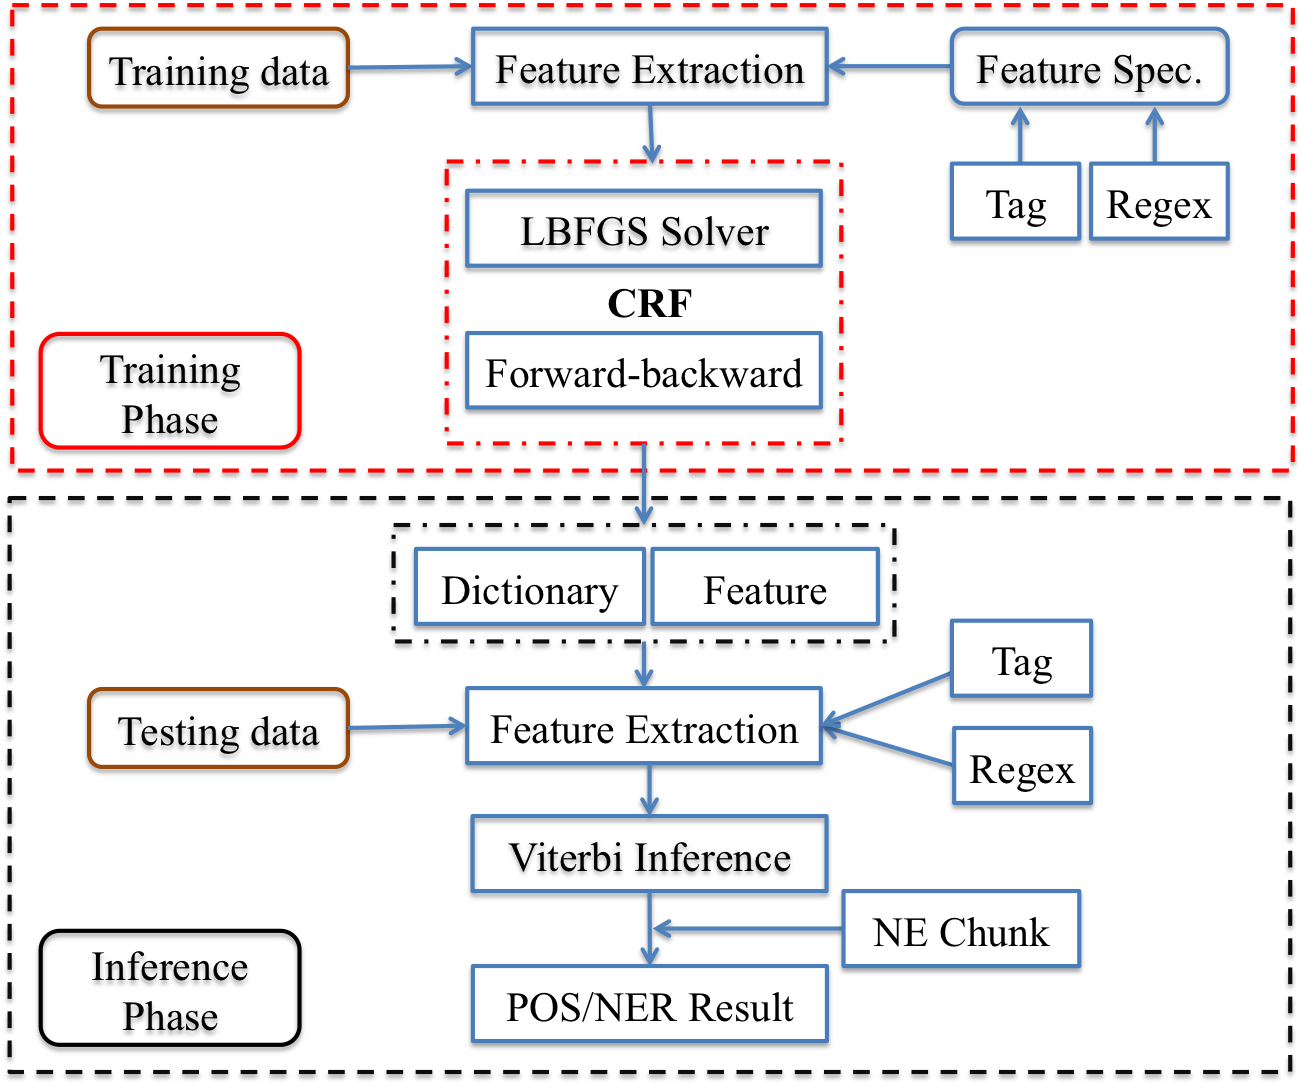
\includegraphics[height=15em]{system.png}
\end{center}

\subsection{Part-of-speech Tagging}
Part-of-speech tagging, also called grammatical tagging or word-category disambiguation is the process of assigning 
a part of speech to each word in a sentence. POS has been widely used in information retrieval and text to speech. 
There are two distinct methods for 
POS task: rule-based and stochastic.
In rule-based method, large collection of rules are defined to indentify the tag. Stochastic method is based on 
probabilistic graphic models such as hidden markov models and conditional random fields. In practice, 
conditional random fields are approved to achieve the state of art accuracy.

\subsubsection{Feature Extraction}
The Feature Extraction module provides functionality for basic text-analysis
tasks such as part-of-speech (POS) tagging and named-entity resolution.
At present, six feature types are implemented.
\begin{itemize}
\item Edge Feature: transition feature that encodes the transition feature weight from current label to next label.
\item Start Feature: fired when the current token is the first token in a sentence.
\item End Feature: fired when the current token is the last token in a sentence.
\item Word Feature: fired when the current token is observed in the trained dictionary.
\item Unknown Feature: fired when the current token is not observed in the trained dictionary for at least certain times.
\item Regex Feature: fired when the current token can be matched by the regular expression.
\end{itemize}

Advantages of extracting features using SQL statements:
\begin{itemize}
\item [$\star$] Decoupling the feature extraction and other code.
\item [$\star$] Compared with procedure language, SQL is much more easier to understand.
\item [$\star$] Storing all the features in tables avoids recomputing of features over iterations. It also boosts the performance.
\item [$\star$] SQL is naivelly paralleled.
\end{itemize}

\begin{itemize}
\item $SQL_1$:\\
\begin{lstlisting}[language=SQL,gobble=4]
    SELECT doc2.start_pos, doc2.doc_id, 'E.', ARRAY[doc1.label, doc2.label]
    FROM   segmenttbl doc1, segmenttbl doc2
    WHERE  doc1.doc_id = doc2.doc_id AND doc1.start_pos+1 = doc2.start_pos
\end{lstlisting}

\item $SQL_2$:\\
\begin{lstlisting}[language=SQL,gobble=4]
    SELECT start_pos, doc_id, 'R_' || name, ARRAY[-1, label]
    FROM  regextbl, segmenttbl
    WHERE seg_text ~ pattern
\end{lstlisting}
\end{itemize}

\paragraph{Build the feature dictionary and assign each feature with a unique feature id}
\begin{itemize}
\item $SQL_3$\\ 
\begin{lstlisting}[language=SQL,gobble=4]
    INSERT INTO tmp_featureset(f_name, feature) 
    SELECT DISTINCT f_name, feature
    FROM   tmp1_feature;
    INSERT INTO featureset(f_index, f_name, feature) 
    SELECT nextval('seq')-1, f_name, feature
    FROM   tmp_featureset;
\end{lstlisting}
\end{itemize}

\paragraph{Generate sparse\_r table}
\begin{itemize}
\item $SQL_3$\\ 
\begin{lstlisting}[language=SQL,gobble=4]
    INSERT INTO rtbl(start_pos,doc_id,feature)
    SELECT start_pos, doc_id, array_cat(fset.feature, 
			ARRAY[f_index,start_pos, 
			CASE WHEN tmp1_feature.feature = fset.feature THEN 1
			ELSE 0 END] )
    FROM   tmp1_feature, featureset fset
    WHERE  tmp1_feature.f_name = fset.f_name AND fset.f_name <> 'E.';
\end{lstlisting}
\end{itemize}


\subsubsection{Parallel Linear-chain CRF Training}
\begin{algorithm} 
\caption{CRF training$(z_{1:M})$} \label{alg:CRF training}
\alginput{Observation set $z_{1:M}$,\\
convergence criterion $\mathit{Convergence}()$,\\
start strategy $\mathit{Start}()$,\\
initialization strategy $\mathit{Initialization}()$,\\
transition strategy $\mathit{Transition}()$,\\
finalization strategy $\mathit{Finalization}()$}
\algoutput{Coefficients $w \in R^N$}
\algprecond{$iteration = 0, diag = 1$}
\begin{algorithmic}[1]
\State $w_{new} \gets \mathit{Start}(z_{1:M})$
\Repeat
        \State $w_{old} \gets w_{new}$
        \State $\mathit{state} \gets \mathit{Initialization}(w_{new})$
\For{$m \in 1..M$} \Comment{Single entry in the observation set}
\State $\mathit{state} \gets \mathit{Transition}(\mathit{state}, z_m)$
                \Comment{Computing gradient and log-likelihood.}
\EndFor
\State $w_{new} \gets Finalization(\mathit{state})$ \Comment{Mainly invoke L-BFGS convex solver}
\Until{$Convergence(w_{new}, g_{new}, \mathit{iteration})$}
    \State \Return $w_{new}$
\end{algorithmic}
\end{algorithm}

\paragraph{Programming Model.}
We provide above the algorithm of parallel CRF training strategy, in the fashion of the selected programming model supported by MADlib (mainly user-defined aggregate).

\paragraph{Parallelism.}
The outer loop is inherently sequential over multiple iterations.
The iteration $n+1$ takes the output of iteration $n$ as input, so on so forth until the stop criterion is satisfied.
The inner loop which calculates the gradient and log-likelihood for each document is data-parallel.
Simple model averaging are used to merge two states.
A merge function is not explicitly added to the pseudocode for simplicity.
The finalization function invokes the L-BFGS convex solver to get a new solution. L-BFGS is sequential, but very fast.
Experiments show that the speed-up ration approaches the number of segments configured in the Greenplum database.

\paragraph{Convergence criterion.}
Usually, the following conditions are combined by AND, OR, or NOT.
\begin{enumerate}
    \item The norm of gradient divided by the norm of coefficient drops below a given threshold.
    \item The maximum number of iterations is reached.
    \item There could be more.
\end{enumerate}

\paragraph{Start strategy.}
In most cases, zeros are used unless otherwise specified.

\paragraph{Transition strategies.}
This function contains the logic of computing the gradient and log-likelihood for each tuple using the forward-backward
algorithm. The algorithms will be discussed in the following sections.

\begin{algorithm}
\caption{transition-lbfgs$(\mathit{state}, z_m)$} \label{alg:transition-lbfgs}
\alginput{Transition state $\mathit{state}$,\\
observation entry $z_m$,\\
gradient function $\mathit{Gradient}()$}
\algoutput{Transition state $\mathit{state}$}
\begin{algorithmic}[1]
    \State $\{state.g,state.loglikelihood\} \gets \mathit{Gradient}(\mathit{state}, z_m)$
        \Comment{using forward-backward algorithm to calculate gradient and loglikelihood}
    \State $\mathit{state}.num\_rows \gets \mathit{state}.num\_rows + 1$
    \State \Return $\mathit{state}$
\end{algorithmic}
\end{algorithm}


\paragraph{Merge strategies.}
The merge function simply sums the gradient and log-likelihood over all training documents
\begin{algorithm}
\caption{merge-lbfgs$(\mathit{state_1}, \mathit{state_2})$} \label{alg:merge-lbfgs}
\alginput{Transition state $\mathit{state_1}$,\\
Transition state $\mathit{state_2}$}
\algoutput{Transition state $\mathit{state_{new}}$}
\begin{algorithmic}[1]
    \State $\mathit{state_{new}}.g \gets \mathit{state_1}.g + \mathit{state_2}.g$
    \State $\mathit{state_{new}}.loglikelihood \gets \mathit{state_1}.loglikelihood + \mathit{state_2}.loglikelihood$
    \State \Return $\mathit{state_{new}}$
\end{algorithmic}
\end{algorithm}


\paragraph{Finalization strategy.}
The finalization function invokes the L-BFGS convex solver to get a new coefficent vector.\\

\begin{algorithm}
\caption{finalization-lbfgs$(state)$} \label{alg:CRF training}
\alginput{Transition state $state$,\\
LBFGS $\mathit{lbfgs}()$}
\algoutput{Transition state $state$}
\begin{algorithmic}[1]
        \State $\{state.g,state.loglikelihood\} \gets penalty(state.g,state.loglikelihood)$ \Comment{To avoid overfitting, add penalization}
        \State $\{state.g,state.loglikelihood\}\gets-\{state.g,state.loglikelihood\}$ \Comment{negation for maximization}
        \State LBFGS instance($state)$ \Comment{initialize the L-BFGS instance with previous state}
        \State instance.$lbfgs()$ \Comment{invoke the L-BFGS convex solver}
        \State instance.save\_state$(state)$ \Comment{save updated variables to the state for next iteration}
        \State \Return $state$
\end{algorithmic}
\end{algorithm}

Feeding with current solution, gradient, log-likelihood, etc., the L-BFGS will ouput a new solution.
To avoid overfitting, a penalization function is needed. We choose to penalize the log-likelihood with a spherical Gaussian weight prior.
Also, L-BFGS is to maximum objective, so we need to negate the gradient vector and log-likelihood to fit our needs in order minimize the log-likehood.

\paragraph{LBFGS Convex Optimization}
The limited-memory BFGS(L-BFGS) is the limited memory variation of the Broyden-Fletcher-Goldfarb-Shanno(BFGS) algorithm which
is the state of art of large scale non constraint convex optimization method.
We translate the in-memory Java implementation to C++ in-database implementation using Eigen support.
Eigen vector and Eigen matrix are used instead of the plain one dimentional and two dimentional arrays.
In the Java in-memory implementation, it defines many static variables defined and shared between the interations.
However, in the MADlib implementation, we define these variables in the state object.
Before each iteration of L-BFGS optimization, we need to initialize the L-BFGS with the current state object. 
At the end of each iteration, we need to dump the updated variables to the database state for next iteration.

\begin{lstlisting}[language=SQL,gobble=4]
    select crf_train_data('/path/to/trainingdataset')
\end{lstlisting}

\begin{lstlisting}[language=SQL,gobble=4]
    select crf_train_fgen('train_segmenttbl', 'crf_regex','crf_dictionary', 
    'featuretbl','crf_feature_dic')
\end{lstlisting}

\begin{lstlisting}[language=SQL,gobble=4]
    select lincrf('featuretbl','spars_r','dense_m','sparse_m','f_size',45, 
    'crf_feature_dic','crf_feature',20)
\end{lstlisting}

\subsubsection{Parallel Linear-chain CRF Inference}
 The Viterbi algorithm is to find the top-k most likely labelings of a document 
for CRF models. 
We chose to implement a Python UDF that uses iterations to drive the Viterbi inference. 
In Greenplum, Viterbi can be run in parallel over different subsets 
of the document on a multi-core machine.

The $vcrf\_top\_label$ is implemented sequentially and each function call will finish labeling of one document. 
The inference is paralledl in the level of document. We use a SQL statment to drive the inference of all documents.
So, the CRF inference is naivelly parallel. 
\begin{lstlisting}[language=SQL,gobble=4]
        SELECT doc_id, vcrf_top1_label(mfactors.score, rfactors.score)
        FROM   mfactors,rfactors
\end{lstlisting}

\paragraph{Inference}
\begin{lstlisting}[language=SQL,gobble=4]
    select crf_test_data('/path/to/testingdataset')
\end{lstlisting}

\begin{lstlisting}[language=SQL,gobble=4]
    select crf_test_fgen('test_segmenttbl',
    'crf_dictionary','crf_label','crf_regex',
    'crf_feature','viterbi_mtbl','viterbi_rtbl')
\end{lstlisting}

\begin{lstlisting}[language=SQL,gobble=4]
    select vcrf_label('test_segmenttbl', 
    'viterbi_mtbl','viterbi_rtbl',
    'crf_label','extraction')
\end{lstlisting}

\cite{DBLP:conf/icml/LaffertyMP01}
\cite{DBLP:journals/scholarpedia/Viterbi09}
\cite{DBLP:journals/siamjo/MoralesN00}
\cite{DBLP:journals/coling/DeRose88}
\cite{DBLP:conf/naacl/ShaP03}
\cite{DBLP:journals/coling/MarcusSM94}


%\begin{thebibliography}{}
%$\[
%V(i,y) =
%\begin{cases}
%\max_{y^\prime}(V(i-1,y^\prime)) + \textstyle \sum_{k=1}^K \lambda_kf_k(y,y^\prime,x_i), & \text{if } i\ge0 \\
%0, & \text{if } i=-1.
%\end{cases}
%\]$

\subsection{Entity Detection}

\section{Performance Evaluation}
\label{sec:length}

\subsection{Scalability}
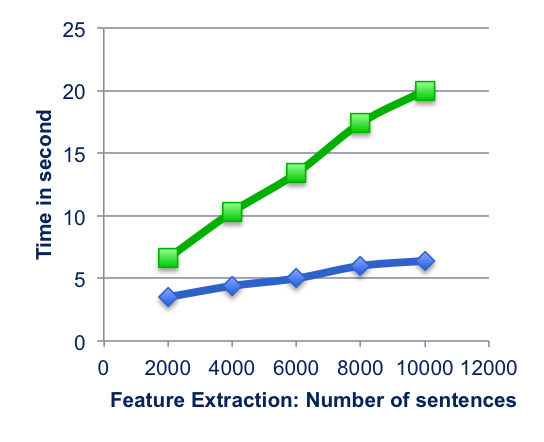
\includegraphics[height=9.9em,width=10em]{extraction.png}
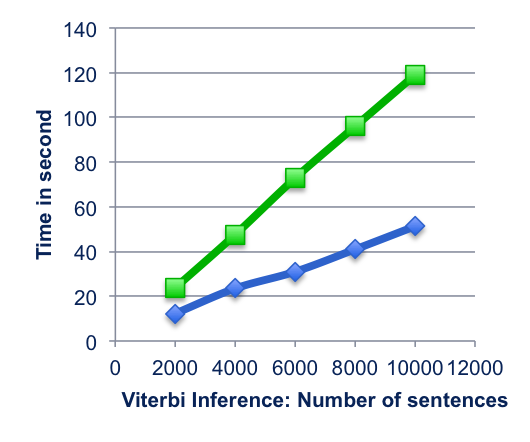
\includegraphics[height=9.9em,width=10em]{viterbi.png}

\subsection{Comparisons with the State of Art}
Compared with PCRF, CRF++

\section{User Case: Tweet Analysis}
\label{sec:blind}


\section*{Acknowledgments}
Christan Grant is funded by a National
Science Foundation Graduate Research Fellowship under Grant No. DGE-0802270.
This work was supported by a gift from EMC Greenplum.

\bibliographystyle{plain}
\bibliography{citation}

\end{document}
